\documentclass{beamer}
%Information
\title{Geometry 1: Triangle}
\titlegraphic{\hfill
\includegraphics[height=1cm]{orange.png}}
\institute{Youth STEM Academy}
\author{Erzhuo Wang}
\date{July 10,2024}
%Theme
\usetheme[block=fill, sectionpage=none]{metropolis}
\useoutertheme{infolines}
\useinnertheme{metropolis}
\setbeamertemplate{blocks}[rounded][shadow=false]
\setbeamertemplate{items}[ball]
\setbeamertemplate{sections/subsections in toc}[ball]
\setbeamertemplate{headline}{}
\logo{YSA}
\usecolortheme{custom}

%Setting
\usepackage[UTF8,noindent]{ctexcap}
\theoremstyle{definition}
\newtheorem{defn}{Definition}[section]
\newtheorem{coro}[defn]{Corollary}
\newtheorem{theo}[defn]{Theorem}
\newtheorem{exer}[defn]{Exercise}
\newtheorem{rema}[defn]{Remark}
\newtheorem{lem}[defn]{Lemma}
\newtheorem{prop}[defn]{Proposition}
\newtheorem{nota}[defn]{Notation}
\newtheorem{exam}[defn]{Example}
\newtheorem{ques}[defn]{Question}

\newenvironment{prooff}{{\noindent\it\textcolor{cyan!40!black}{Proof}:}\,}{\par}
\newenvironment{proofff}{{\noindent\it\textcolor{cyan!40!black}{Proof of the lemma}:}\,}{\qed \par}
\newcommand{\bbrace}[1]{\left\{ #1 \right\} }
\newcommand{\bb}[1]{\mathbb{#1}}
\newcommand{\p}{^{\prime}}
\renewcommand{\mod}[1]{(\text{mod}\,#1)}
\newcommand{\blue}[1]{\textcolor{blue}{#1}}
\newcommand{\spec}[1]{\text{Spec}({#1})}
\newcommand{\rarr}[1]{\xrightarrow{#1}}
\newcommand{\larr}[1]{\xleftarrow{#1}}
\newcommand{\emptyy}{\underline{\quad}}
\newenvironment{enu}{\begin{enumerate}[(1)]}{\end{enumerate}}
%ctrl+点击文本返回代码  选中代码 ctrl+alt+j 为代码查找文本
\begin{document}
\begin{frame}
    \titlepage
\end{frame}
\begin{frame}{Congrent and Similar}
    Two geometry objects are congruent if one can be transormed into the other by a sequence of translations, rotations and reflections.

    如果一个几何图形可以通过一系列的平移、旋转和反射变换成另一个几何图形,那么两个几何图形是全等的。

    Two  geometry objects are similar if one can be dilated by a fixed non-zero constant factor in all dirctions so that it becomes congrent to the other.

    两个几何图形相似是指其中一个可以放大或缩小一个某个非零常数倍, 使得两个几何图形全等.
\end{frame}
\begin{frame}{Congruence(同构)}
    \begin{theo}
        Two triangles are congruent if they satisfy one of the following conditions:
        \begin{itemize}
            \item (SSS): the three sides of one are equal to the three sides of the other.
            \item (SAS): two sides and the included angle of one are equal to two sides and the included angle of the other.
            \item (ASA): two angles and an included side of one are equal to two angles and the included side of the other.
        \end{itemize}
    \end{theo}
\end{frame}
\begin{frame}{Similarity(相似)}
    \begin{theo}[相似三角形对应边成比例]
        Two triangles are similar if and only if two angles of a triangle are equal to two angles of the other triangle. Similar triangles have proportional sides, so if $\triangle A B C \sim \triangle D E F$, then
        $$
            \frac{A B}{D E}=\frac{B C}{E F}=\frac{A C}{D F}
        $$
        is the ratio of similarity.
    \end{theo}
\end{frame}
\begin{frame}{Angle Bisector(角平分线)}
    \begin{theo}[角平分线的等价定义]
        If $D$ is a point on the side $\overline{A C}$ of a triangle $A B C$, then $\overline{B D}$ bisects $\angle A B C$ if and only if
        $$
            \frac{A D}{C D}=\frac{A B}{B C} \text {. }
        $$
    \end{theo}
\end{frame}
\begin{frame}{Pythagorean Theorem(勾股定理)}
    \begin{theo}[直角边的平方等于斜边平方之和]
        If a right triangle has legs with length $a$ and $b$ and hypotenuse with length $c$, then
        \begin{equation*}
            c^2=a^2+b^2
        \end{equation*}
    \end{theo}
\end{frame}
\begin{frame}{Special triangles}
    \begin{theo}
        一个等腰直角三角形, 两腰对应的角度均为$45^\circ$, 腰长与斜边长之比为$1:\sqrt{2}$.

        一个直角三角形, 两腰对应的角度均为$30^\circ$和$60^\circ$, 则$30^\circ$对应的直角边$:60^\circ$对应的直角边:斜边= $1:\sqrt{3}:2$
    \end{theo}
    \begin{figure}
        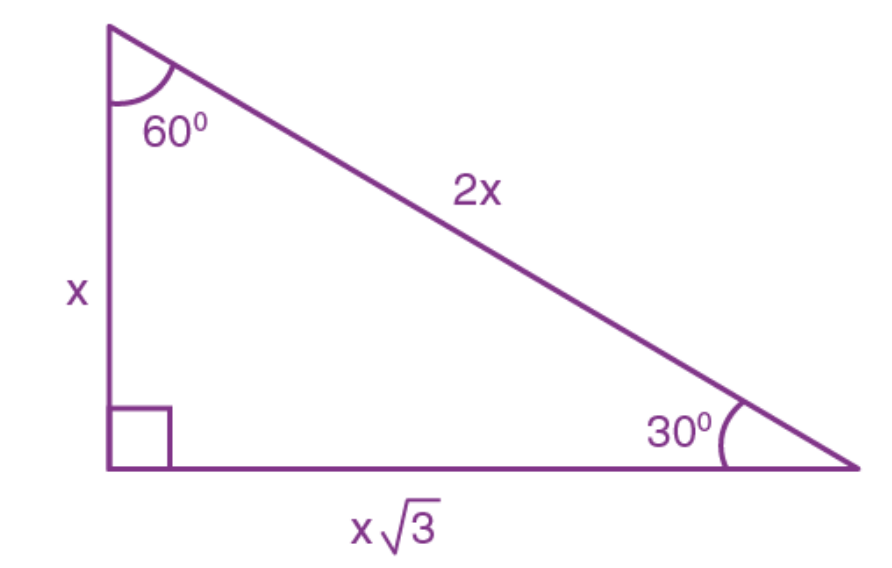
\includegraphics[height=0.4\textheight]{306090.png}
    \end{figure}
\end{frame}
\begin{frame}{Ratio}
    \begin{theo}
        如图$S_1,S_2,S_3,S_4$
        分别为$BDE,BEA,ECA,EDC$的面积,
        若 $\frac{B D}{D C}=\lambda$,
        则 $$\frac{S_1}{S_4}=\frac{S_2}{S_3}=\frac{S_1+S_2}{S_3+S_4}=\lambda$$
    \end{theo}
    \begin{figure}
        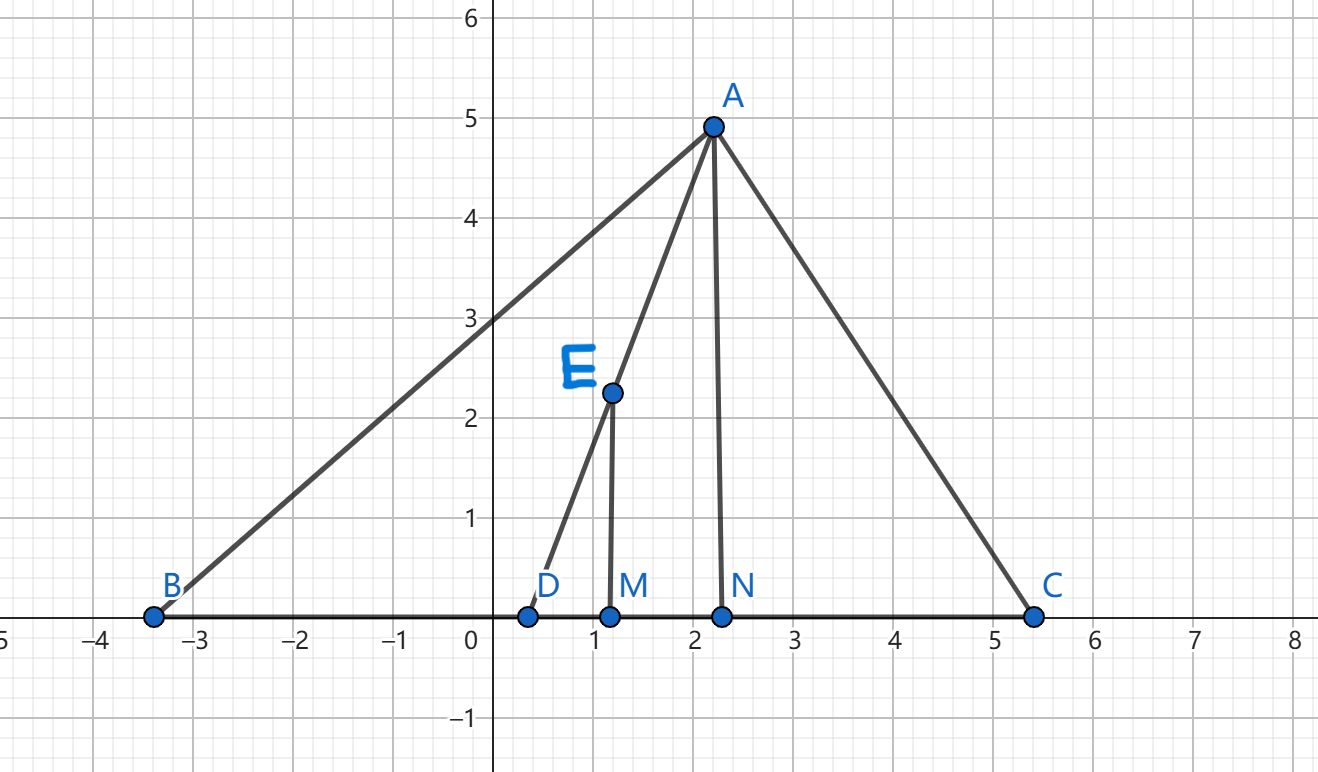
\includegraphics[height=0.4\textheight]{triangle3.png}
    \end{figure}
\end{frame}
\begin{frame}{Exercise}
    \begin{ques}[AMC 8, 2020-25]
        $S_1,S_2,S_3$为三个正方形, 大矩形长$3322$, 宽$2020$, 求$S_2$边长.
        \begin{figure}
            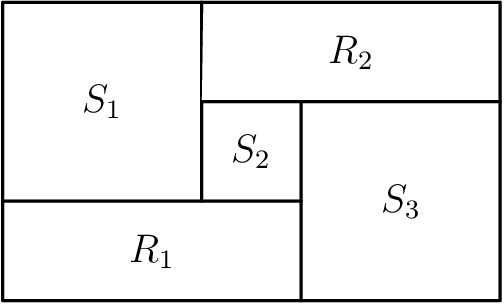
\includegraphics[height=0.4\textheight]{rectangle1.png}
        \end{figure}
    \end{ques}
\end{frame}
\begin{frame}
    \begin{prooff}
        过 $A$ 作 $B C$中垂线交$B$于$M$, 过$E$作$BC$垂线交$BC$于$N$

        则
        $$\frac{S_1}{S_4}=\frac{\frac{1}{2} B D \times E N}{\frac{1}{2} D C \times E N}=\frac{B D}{P C}=\lambda$$
        $$
            \frac{S_1+S_2}{S_3+S_4}=\frac{\frac{1}{2} B D \times A M}{\frac{1}{2} D C \times A M}=\frac{B D}{D C}=\lambda
        $$

        从而,$S_1+S_2=\lambda S_3+\lambda S_4$, 两边消去$S_1=\lambda S_4$得到$S_2=\lambda S_3 \Rightarrow \frac{S_2}{S_3}=\lambda$.

    \end{prooff}
\end{frame}
\begin{frame}{Two Mountains(AMC 8, 2022-24)}
    如下图, 阴影部分面积为$183$, 求$h$.
    \begin{figure}
        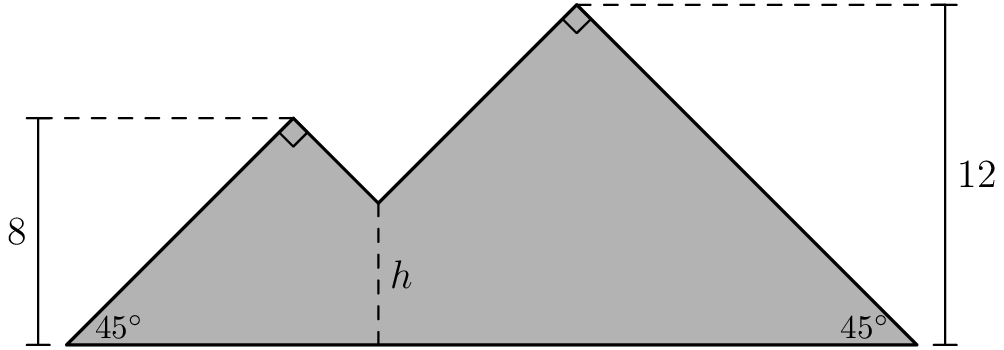
\includegraphics[height=0.4\textheight]{two mountains.png}
    \end{figure}
\end{frame}

\begin{frame}{Angle Bisector}
    Nondegenerate triangle $ABC$ integer sider length, $BD$ is an angle bisector, $AD=3$, $DC=8$. What is
    the smallest possible value of the perimeter?

    三角形$ABC$三边长均为整数, BD为$\angle ABC$的角平分线, $AD=3,DC=8$. 求该三角形周长的最小值.
\end{frame}
\begin{frame}
    \begin{ques}
        In square $ABCE$, $AF=2FE$ and $CD=2DE$. What is the ratio of the area of $\triangle BFD$ to the area of square $ABCE$?
    \end{ques}
    \begin{figure}
        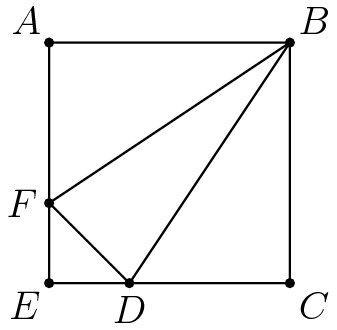
\includegraphics[height=0.4\textheight]{triangle5.png}
    \end{figure}
\end{frame}
\begin{frame}{Homework}
    \begin{ques}[AMC 8, 2023-19]
        如图, 有两个等边三角形, 内三角形为外三角形向着中心点收缩一定比例, 使得内三角形边长为外三角形边长的$\frac{2}{3}$, 求梯形和外三角形面积之比.
        \begin{figure}
            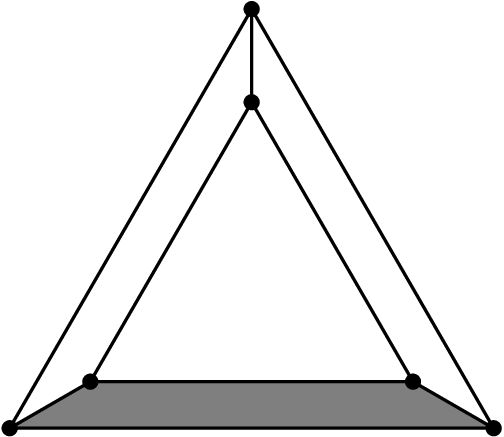
\includegraphics[height=0.4\textheight]{triangle1.png}
        \end{figure}
    \end{ques}
\end{frame}

\end{document}